\documentclass{article}
\textheight 22.5truecm \textwidth 14.5truecm
\setlength{\oddsidemargin}{0.35in}\setlength{\evensidemargin}{0.35in}

\usepackage[utf8]{inputenc}
\usepackage[russian]{babel}
\usepackage{graphicx}
\usepackage{amsmath}
\usepackage{breqn}
\usepackage{wrapfig}
\usepackage{float}
\usepackage{multirow}
\usepackage{caption}
\usepackage{subcaption}

\graphicspath{ {./data/images} }
\author{Александр Романов Б01-110}
\date{}
\title{2.2 Изучение спектров водорода и дейтерия}

\begin{document}
\maketitle
\section{Введение}
\subsection{О работе}
Исследуются спектральные закономерности в оптических спектрах водорода и дейтерия.
По результатам измерений вычисляются постоянные Ридберга для этих двух изотопов
водорода, их потенциалы ионизации, изотопические сдвиги линий.
\subsection{Схема установки}
\begin{figure}[H]
	\centering
	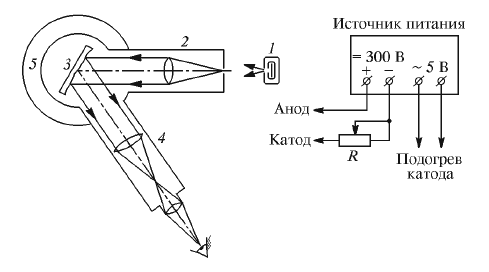
\includegraphics[width=0.7\textwidth]{scheme.png}
\end{figure}
\section{Работа}
\subsection{Каллибровка установки}
Откалибруем установку по спектру неона:
\begin{table}[H]
	\centering
\begin{tabular}{|c|c|c|}
	\hline
lambda, units & lambda, A & num \\\hline
2574          & 7032.41   & 1   \\\hline
2562          & 6929.47   & 2   \\\hline
2480          & 6717.04   & 3   \\\hline
2478          & 6678.28   & 4   \\\hline
2444          & 6598.95   & 5   \\\hline
2414          & 6532.88   & 6   \\\hline
2412          & 6506.53   & 7   \\\hline
2373          & 6402.24   & 8   \\\hline
2364          & 6382.99   & 9   \\\hline
2342          & 6334.42   & 10  \\\hline
2332          & 6304.79   & 11  \\\hline
2320          & 6266.49   & 12  \\\hline
2296          & 6217.28   & 13  \\\hline
2280          & 6163.59   & 14  \\\hline
2266          & 6143.06   & 15  \\\hline
2248          & 6096.14   & 16  \\\hline
2238          & 6074.34   & 17  \\\hline
2226          & 6030      & 18  \\\hline
2194          & 5975.53   & 19  \\\hline
2180          & 5944.83   & 20  \\\hline
2150          & 5881.89   & 21  \\\hline
2132          & 5852.49   & 22  \\\hline
1874          & 5400.56   & 23  \\\hline
\end{tabular}
	\caption{Спектр неона}
\end{table}

И также по спектру ртути

\begin{table}[H]
	\centering
\begin{tabular}{|c|c|c|}
	\hline
lambda, units & lambda, A & num \\\hline
2540          & 6907      & K1  \\\hline
2308          & 6234      & K2  \\\hline
2100          & 5791      & 1   \\\hline
2090          & 5770      & 2   \\\hline
1912          & 5461      & 3   \\\hline
1494          & 4916      & 4   \\\hline
734           & 4358      & 5   \\\hline
292           & 4047      & 6   \\\hline
\end{tabular}
	\caption{Спектр ртути}
\end{table}
\subsection{Спектр водорода}
Теперь перейдём к измерению водорода

\begin{table}[H]
	\centering
\begin{tabular}{|c|c|}
	\hline
lambda, units & num \\\hline
2428          & 0   \\\hline
1440          & 1   \\\hline
806           & 2   \\\hline
\end{tabular}
	\caption{Спектр водорода}
\end{table}

Учтя каллибровку

\begin{table}[H]
	\centering
\begin{tabular}{|c|c|}
	\hline
lambda, A & num \\\hline
6556 & 0 \\\hline
4976 & 1 \\\hline
4439 & 2 \\\hline
\end{tabular}
	\caption{Спектр водорода}
\end{table}

\subsection{Спектр Йода}
Несколько изменим установку

\begin{figure}[H]
	\centering
	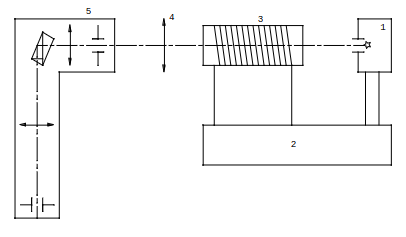
\includegraphics[width=0.7\textwidth]{scheme-iodine.png}
\end{figure}

\begin{table}[H]
	\centering
\begin{tabular}{|c|c|}
	\hline
lamda, units & num							\\\hline
	2374         & \(h\nu_{1,0}\) \\\hline
2262         &  \(h\nu_{1,5}\)	\\\hline
2584         & left							\\\hline
572          & right						\\\hline
\end{tabular}
	\caption{Спектр Йода}
\end{table}

\begin{table}[H]
	\centering
\begin{tabular}{|c|c|}
	\hline
lambda, A         & num \\\hline
6428 & \(h\nu_{1,0}\)   \\\hline
6162 & \(h\nu_{1,5}\)   \\\hline
6927 & left					    \\\hline
4242 & right						\\\hline
\end{tabular}
	\caption{Спектр Йода}
\end{table}

\section{Выводы}
\end{document}
